\subsection{Fonction de plusieurs variables}

\begin{exercice}
\begin{enumerate}
\item Soit $u(x,y)$ la fonction définie par 
$$u(x,y) = x^2+xy +x-2y^2+2y$$
et  les deux sous-ensembles de de $\R^2$, $E$ et $F$ définies par : 
$$E = \{ (x,y) \in \R_2 \, | \,  -\frac{x}{2} \leq  y  \leq x+1\}\quad \quad F = \{ (x,y) \in \R_2 \, | \, x+1 \leq  y  \leq - \frac{x}{2}\}$$

\begin{enumerate}
\item Sur un graphique soigné,  représenter $E$ et $F$. 
\item En considérant à $y$  fixé, la fonction polynômiale $P(x) = u(x,y)$, résoudre $u(x,y)\geq 0$\\
\end{enumerate}
\item   Soit $f$ la fonction définie par  $$f(x,y) = \int_{0}^{u(x,y) }e^{\sqrt{t}}\,  dt.$$
\begin{enumerate}
\item Déterminer l'ensemble de définition de $f$. 
\item Caculer le gradient de $f$.
\item En déduire que $\left(\frac{-2}{3},\frac{1}{3}\right)$ est l'unique point critique de $f$. 
\end{enumerate}
\item 
\begin{enumerate}
\item Calculer $f\left(\frac{-2}{3},\frac{1}{3}\right)$.
\item Montrer que $\left(\frac{-2}{3},\frac{1}{3}\right)$ est un minimum sur l'ensemble de définition de $f$. 
\item Question bonus  : D'autres points réalisent ce minimum, lesquels ? Pourquoi le gradient ne s'annule pas en ces autres points ? 
\end{enumerate}
\end{enumerate}
\end{exercice}



\begin{correction}
\begin{enumerate}
\item \begin{enumerate}
\item Tracer en python ; \begin{center}
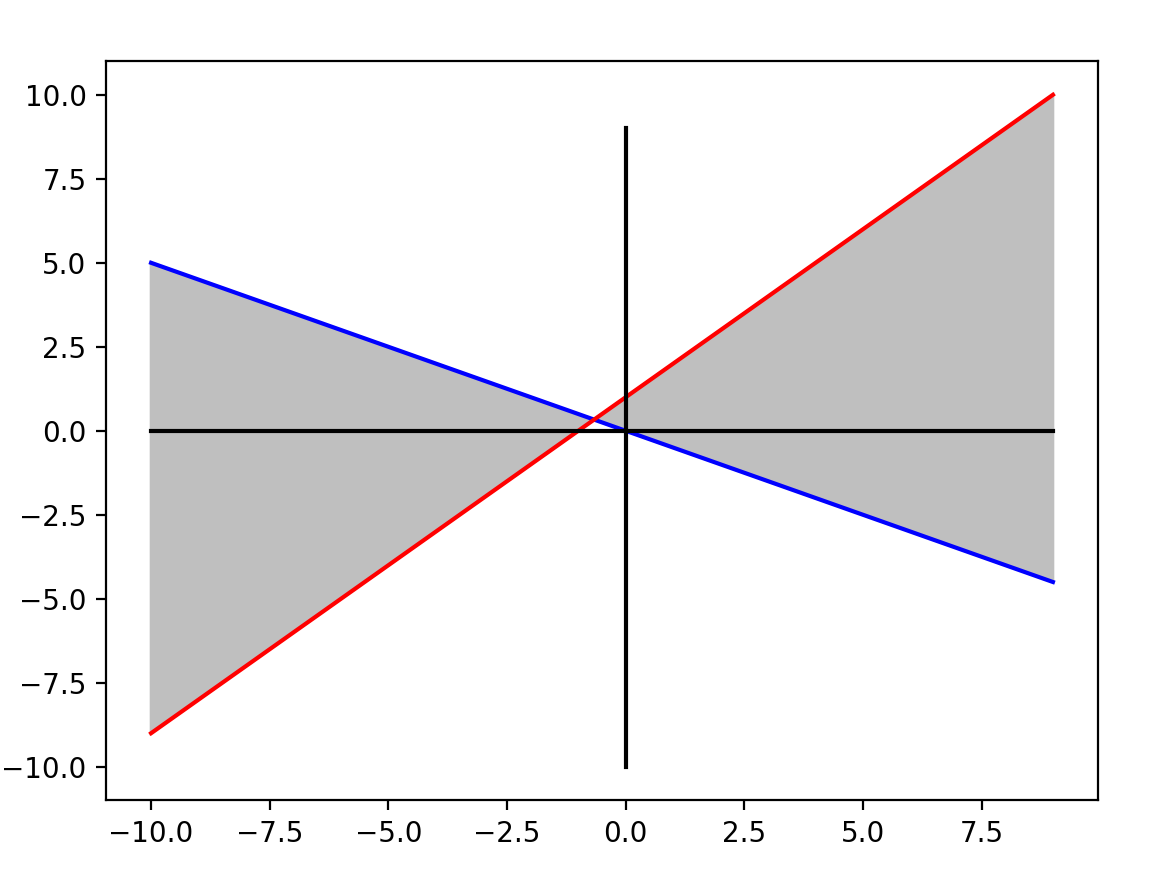
\includegraphics[scale=0.4]{EetF.png}
\end{center}
\begin{lstlisting}
import matplotlib.pyplot as plt
import numpy as np
plt.clf()
X=np.arange(-10,10,1)
Y=-X/2

plt.plot(X,Y,'b')
plt.plot(X,X+1,'R')
plt.plot(X,0*X,'black')
plt.plot(0*X,X,'black')

plt.fill([-2/3,9,9],[1/3,-4.5,10],color = '0.75')
plt.fill([-2/3,-10,-10],[1/3,5,-9],color = '0.75')
plt.show()
\end{lstlisting}
\item Ecrivons $P(x)$ sous la forme bien connue d'un polynôme du second degré : $P(x) = x^2 +x(y+1) -2y^2+2y$. On calcule son discriminant on obtient 
$$\Delta = (y+1)^2 -4 (-2y^2+2y) = 9y^2 - 6y +1= (3y-1)^2\geq 0$$
On obtient donc deux racines réelles (possiblement confondues) 
$$\frac{-y-1 \pm|3y-1|}{2} $$
$$-2y  \quadet  y-1$$
On peut donc écrire 
$$P(x) = (x+2y) (x-y+1)$$
Comme $y$ est arbitraire on obtient pour tout $(x,y) \in \R^2$, $$u(x,y) = (x+2y) (x-y+1)$$

Ainsi, $u(x,y) \geq 0$ si et seulement 

$$\left\{ 
\begin{array}{cc}
x+2y &\geq 0\\
x-y+1&\geq 0
\end{array}\right. 
\quadou 
\left\{ 
\begin{array}{cc}
x+2y &\leq 0\\
x-y+1&\leq 0
\end{array}\right.$$

$$\left\{ 
\begin{array}{cc}
y &\geq -\frac{x}{2}\\
y&\leq x-1
\end{array}\right. 
\quadou 
\left\{ 
\begin{array}{cc}
y &\leq -\frac{x}{2}\\
y&\geq x-1
\end{array}\right.$$
$$(x,y)\in E \quadou (x,y)\in F$$

Ainsi $$u(x,y)\geq 0 \equivaut (x,y) \in E\cup F$$



\end{enumerate}
\item \begin{enumerate}
\item Notons $g(t) = e^{\sqrt{t}}$. $g$ est définie est continue sur $\R^+$. Ainsi $f$ est bien définie pour tout $(x,y)\in \R^2$ tel que $u(x,y) \geq 0$ c'est-à-dire d'après la question précédente : $(x,y)\in E\cup F$. 
\item On calcule les dérivées partielles. Notons $G$  une primitive de $g$ sur $\R_+$ on  a 
$$f(x,y) = G(u(x,y)) -G(0).$$
Donc 
\begin{align*}
\frac{\partial f}{\partial x} (x,y) &= \frac{\partial u}{\partial x} (x,y) G'(u(x,y))\\
												&= (2x+y +1)e^{u(x,y)}
\end{align*}

et 

\begin{align*}
\frac{\partial f}{\partial y} (x,y) &= \frac{\partial u}{\partial y} (x,y) G'(u(x,y))\\
												&= (x-4y+2) e^{u(x,y)}
\end{align*}
D'où 
$$\nabla f  (x,y) = \left( \begin{array}{c}
 (2x+y +1)e^{u(x,y)}\\
  (x-4y+2) e^{u(x,y)}
\end{array}
\right)$$
\item \begin{align*}
\nabla f = \left( \begin{array}{c}
0\\
0
\end{array}
\right)
\quad &\equivaut\quad  \left( \begin{array}{c}
 (2x+y +1)e^{u(x,y)}\\
  (x-4y+2) e^{u(x,y)}
\end{array}\right) =\left( \begin{array}{c}
0\\
0
\end{array}
\right)\\
&\equivaut \left\{\begin{array}{cl}
2x+y +1&=0\\
x-4y+2&=0
\end{array}\right.\\
&\equivaut \left\{\begin{array}{cl}
x-4y&=-2\\
2x+y&=-1
\end{array}\right.\\
&\equivaut \left\{\begin{array}{ccl}
x&-4y&=-2\\
&9y&=3
\end{array}\right.\\
&\equivaut \left\{\begin{array}{ccl}
x&-4y&=-2\\
&y&=\frac{1}{3}
\end{array}\right.\\
&\equivaut \left\{\begin{array}{cl}
x&=-2+4\frac{1}{3} = \frac{-2}{3}\\
y&=\frac{1}{3}
\end{array}\right.\\
\end{align*}


\end{enumerate}
\item \begin{enumerate}
\item $u\left(\frac{-2}{3},\frac{1}{3}\right) =\left(\frac{-2}{3}\right)^2 +\left(\frac{-2}{3} \frac{1}{3}\right)  -\frac{2}{3}  -2 \left(\frac{1}{3}\right)^2 +2 \frac{1}{3} = 0$. Donc 
$$f\left(\frac{-2}{3},\frac{1}{3}\right) = 0$$
\item Pour tout $(x,y) \in D_f$, $u(x,y) \geq 0$ donc comme pour tout $t\geq 0, $  $e^{\sqrt{t}}>0$ on  a bien 
$$\int_0^{u(x,y)} e^{\sqrt{t}} dt \geq 0$$
et ainsi, $$u(x,y) \geq 0 =f\left(\frac{-2}{3},\frac{1}{3}\right)  $$
\item Tous les points 'au bord' de $E$ et $F$ satisfont $u(x,y)=0$ en effet si 
$x+2y = 0 $ ou $x-y+1=0$ on a bien $u(x,y) =0$ d'après la factorisation obtenue a la question 1b). 
Ces points n'ont pas un gradient nul alors que ce sont aussi des minima... Il n'y a pas de problème car dans le théorème disant "minima $\implique$ gradient nul" il faut que le point soit à \underline{intérieur} du domaine de définition. -
\end{enumerate}
\end{enumerate}

\end{correction}